\section{Introduction}
\label{section_intro}
In this chapter we will relate the integrated path of an asteroid to its appearance to an observer on Earth.
We will review the equatorial coordinate system, which describes the location of an object in the sky 
with the parameters right ascension (RA) and declination (DEC).
We will develop the calculations to transform between a direction from earth represented as a pair (RA, DEC)
to a direction represented as a unit vector $\uvec = (u_x, u_y, y_z)$ in the barycentric mean ecliptic frame.
We will explore the ZTF dataset of telescopic observation from the Palomar observatory in California.
We will compute the direction $\uvec$ from which an observer at Palomar would have seen an object at a given observation time
as a function of its predicted position $\qvec$ and velocity $\vvec$ at that observation time.
This calculation will account for the time required for light to reach the observatory (``light time'')
and for the location of the observatory on the surface of the earth as distinct from geocenter (``topos adjustment'').
We will run this calculation on all the known asteroids, computing the direction they would have appeared in the sky if they had been visible at Palomar.
We will use this calculation to associate each ZTF obervation with the nearest asteroid to it in the sky.

Finally, we will study the statistical distribution of angular distance between the ZTF observations and the nearest asteroid.
We will show that 65.71\% of these observations fall within 2.0 arc seconds of the direction predicted for one of the 733,489 catalogued asteroids.
We will compare this to the theoretical distribution of angular distances to the nearest asteroid 
if the predicted directions were distributed uniformly on the sphere.
We will show that such a high preponderance of ``hits'' is wildly unlikely and conclude that the asteroid catalogue 
has correct orbital elements for the objects being detected, 
and that the combined tolerance of the instruments and this calculation apparatus is on the order of 2.0 arc seconds.

\section{A Brief Review of Right Ascension (RA) and Declination (DEC)}
\label{section_ra_dec}
How can we describe the direction of an object we see in the sky?
It is a question that dates back to the first astronomers in ancient times.
The simplest and most intuitive coordinate system is the \href{https://en.wikipedia.org/wiki/Horizontal_coordinate_system}{topocentric coordinate system},
which uses the local horizon of an observer on the surface of the Earth as the fundamental plane.
In this coordinate system, an object in the sky is described in terms of an altitude (sometimes called an elevation) and an azimuth.
The altitude is how many degrees the object is above the visible horizon, so it will be between $0 \degree$ and $90 \degree$.
The topocentric coordinate system is intuitive and easy to use for an observer standing on the surface of the earth and looking at the sky.
If I wanted to do some amateur astronomy with my kids and know where to point an inexpensive telescope, these are the coordinates I would want.
\begin{figure}[hbt!]
\begin{center}
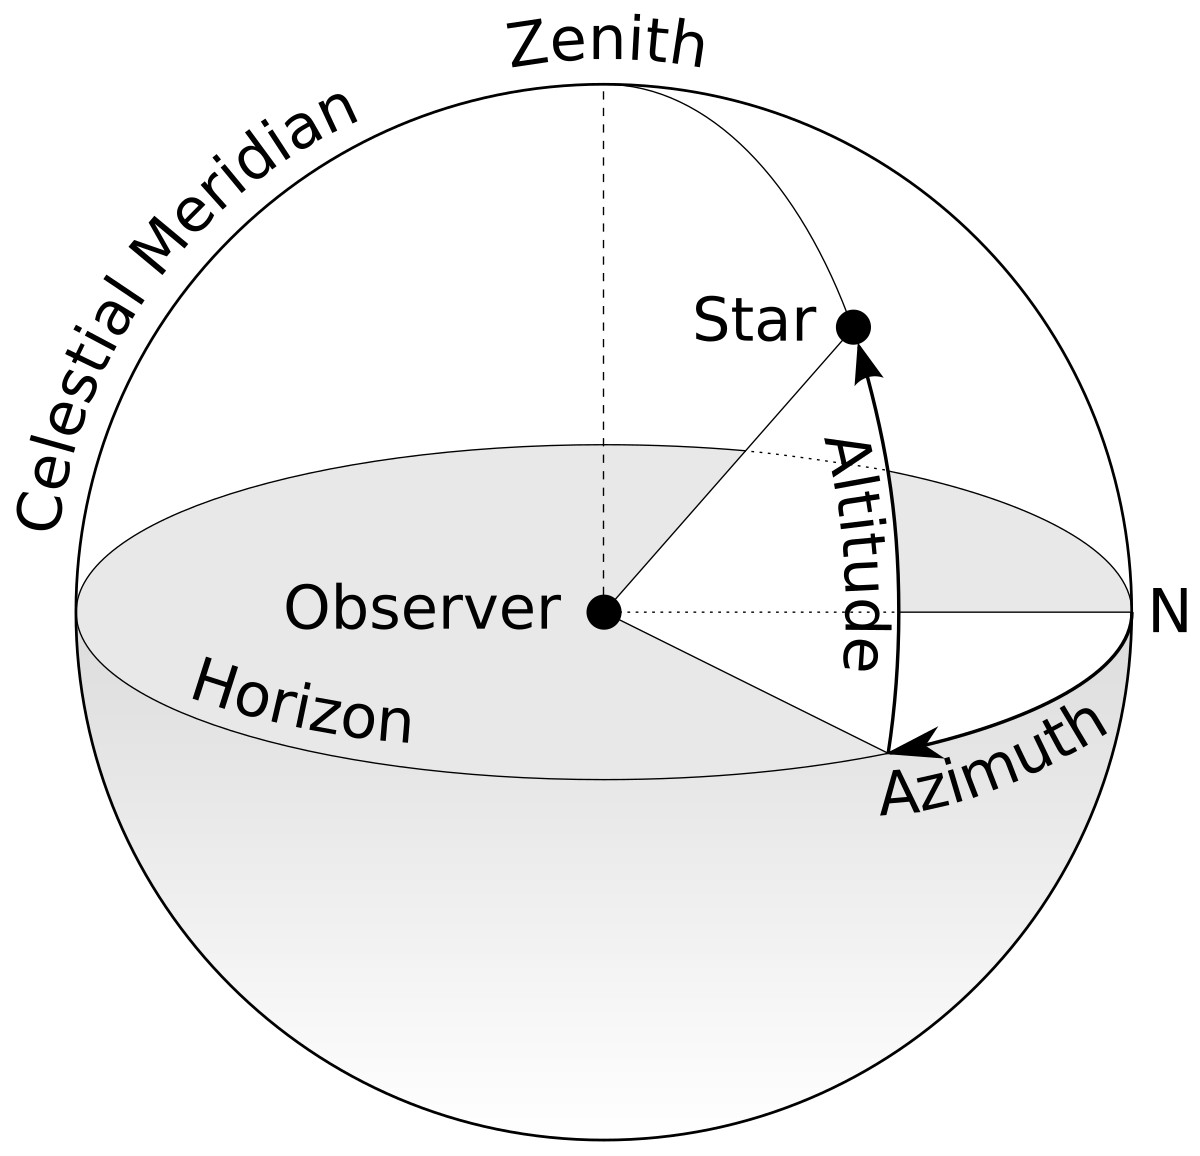
\includegraphics[width=0.6\textwidth]{topocentric_coordinates.png}
\caption{The topographic coordinate system, courtesy of \href{https://en.wikipedia.org/wiki/Horizontal_coordinate_system}{Wikipedia}}
\end{center}
\end{figure}

But the topcentric coordinate system is poorly suited to sharing observational data between astronomers.
It is a different reference frame depending on where you are located on the Earth and the time in the evening.
For this reason, astronomers dating back to ancient times developed the \href{https://en.wikipedia.org/wiki/Equatorial_coordinate_system}{equatorial coordinate system}.
This coordinate system draws an imaginary sphere around the earth.
The $x$ axis of this coordinate frame points from the Sun to the center of the Earth at the Vernal Equinox of a specific date 
(typically \href{https://en.wikipedia.org/wiki/Epoch_(astronomy)}{J2000.0} these days).
The $y$ axis is 90 degrees to the East and the $z$ axis points to the North pole.
This is much easier to understand with a picture than with words:
\begin{figure}[hbt!]
\begin{center}
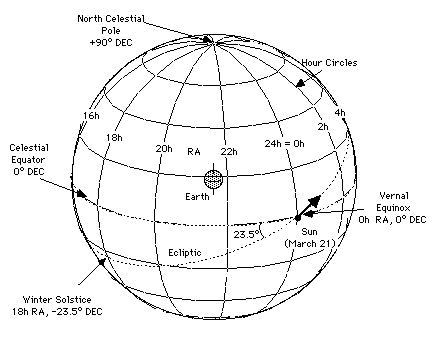
\includegraphics[width=0.8\textwidth]{celestial_sphere.png}
\caption{The celestial sphere, courtesy of \href{http://coolcosmos.ipac.caltech.edu/cosmic_classroom/cosmic_reference/coordsys.html}{cool cosmos}.}
\end{center}
\end{figure}

The celestial sphere was originally conceived as having its $z$ axis pointing along the axis of the Earth's rotation, i.e. from the South Pole to the North Pole.
This is not a good definition though for the purposes of modern astronomy, 
because the Earth's rotational axis is not a fixed direction in the barycentric mean ecliptic frame.
The Earth's rotational axis changes over time due to two separate effects: 
\href{https://en.wikipedia.org/wiki/Axial_precession}{precession} and \href{https://en.wikipedia.org/wiki/Astronomical_nutation}{nutation}.
Precession is a low frequency, predictable effect that in analagous to wobbling movement of a top's rotational axis.
It is typically covered in a first semester undergraduate physics course on mechanics.
The precession of the Earth's axis is caused by mainly by the gravitational influence of the Sun and Moon, and has a period of approximately 25,772 years.
Nutation is a high frequency effect, also caused mainly by the gravitational foreces of the Sun and Moon.
In fact, the only difference bewteen the two effects is in the way we model and understand them.
Precession isolates the mean perturbation over time; it's a slow, steady drift that is easy to predict.
Nutation describes the much smaller, high frequency wobbles (on the order of tens of arc seconds) that are the residual after precession is accounted for.

Because of the instability of the Earth's rotational axis, the definition of the directions were updated to refer to the mean ecliptic as of a date,
rather than Earth's rotational axis when the measurement is taken.
Detailed calculations of the precession and nutation can then be used to adjust measurements taken on different dates.
Ineed, the \tty{astropy} astronomy package has the capability to perform these calculations.
The diagram of the equataorial coordinate system clarifies this more modern definition.  
The vernal equinox is the moment when the Earth's orbit crosses the ecliptic.

This definition of a celestial coordinate system has in turn been superseded by a still more accurate system:
the Interational Celestial Reference System, \href{https://en.wikipedia.org/wiki/International_Celestial_Reference_System}{ICRS}.
The ICRS is based on an elegant idea.
The goal of a celestial reference frame is to provide directions that are as near to fixed as possible in the reference frame of the solar system.
Astronomers realized that since objects that are very far away from the Milky Way have orientations that are effectively fixed,
the most precise way to define directions was based on large quantities of astronomical observations of these objects.
In particular, radioastronomy (observations of stars in the radio wave frequency) is used.
This is the basis of the ICRS and the frame of reference it defines: the International Celestial Refrence Frame (ICRF).
The ICRF is a 3 dimensional coordinate system whose origin is the solar system barycenter (center of mass).
The $X$, $Y$ and $Z$ axes are set by convention to line up very closely to the traditional definition of the J2000.0 frame.
The orientation of the coordinate axes is based on the measured positions of 212 extragalactic objects, mainly quasars.
These objects are so far away from Earth and the Milky Way galaxy that they are considered ``fixed points'' in space.
\footnote{\href{http://kejian1.cmatc.cn/vod/comet/oceans/naval_observatory/navmenu.php_tab_1_page_3.2.1_type_text.htm}{U.S. Naval Observatory - ICRS}}
Modern telescopes can achieve extremely accurate RA/Dec measurements by calibrating against the measured directions to these objects.
\begin{figure}[hbt!]
\begin{center}
\includegraphics[width=0.8\textwidth]{ICRS_USNO.jpg}
\caption{The International Celestial Reference Frame (ICRF), courtesy of 
\href{http://kejian1.cmatc.cn/vod/comet/oceans/naval_observatory/navmenu.php_tab_1_page_3.2.1_type_text.htm}{U.S. Naval Observatory}.}
\end{center}
\end{figure}

The main conclusion of this short section is that even an apparently simple idea, the direction from an observer on Earth to an object seen in the sky,
is quite subtle if you want to take reproducible measurements that are accurate on the order of arc seconds.
The ICRS is accurate on the order of a handful of milliarcseconds, 
meaning that uncertainty in the coordinate frame is not a meaningful contributor to errors for any calculations in this thesis.
Fortunately this is a mature and well studied problem in astronomy, and it is addressed well by the \tty{astropy} package.
Rather than trying to reinvent the wheel, I use the \tty{astropy} as much as possible in the next section
to relate RA/Dec measurements to directions $\uvec$ in the barycentric mean ecliptic frame.

\section{Mapping Between RA/Dec and Direction $\vec{u}$ in the Ecliptic Frame}
\label{section_ra_dec_to_dir}
In the previous section we have explored the ICRS, which provides the definition of the RA/Dec measurements quoted by astronomers.
In this section, I review the definition of the barycentric mean ecliptic frame that is used for all calculations in this thesis.
Then I explain the functions that are used to perform the conversions between RA/Dec and directions in the ecliptic frame.

The barycentric ecliptic frame is the natural choice for computations done in relation to integrations of the solar system.
It defines the $xy$ plane to containing the mean ecliptic (ellipse of the Earth's orbit around the Sun).
We take the mean ecliptic because the ecliptic varies slowly over time; 
the rotation of the Earth around the Sun in any given year would not be contained \textit{exactly} in a plane,
but there is a mean plane that comes closest in the least square sense to hitting all the points.
The $z$ axis is the unique direction that is orthogonal to this plane.
Within the $xy$ plane, the $x$ axis is oriented from the Sun to Earth geocenter at the vernal equinox.
In particular, the $x$ axis is the direction from the Earth to the Sun at the vernal equinox as of the epoch, 
which is currently J2000.0 (JD 2451545.0, approximately January 1, 2000 12:00 UTC on the Gregorian calendar).

Here the vernal equinox is not defined with its ancient interpretation as the day when the day and night have equal lengths,
but by the modern astronomical definition as the intersection of two planes:
the mean ecliptic plane described above, and the mean equator as of that date.
The idea of the mean equator as of a date is that as described above, the Earth's equator undergoes small wobbles at high frequency due to nutation.
The mean equator as of a date disregards these wobbles, and instead considers only the trend of the equator, which changes slowly due to precession.
This definition has the advantages of being more precisely measurable and changing more slowly than the true equator, making it the standard.

\begin{figure}[hbt!]
\begin{center}
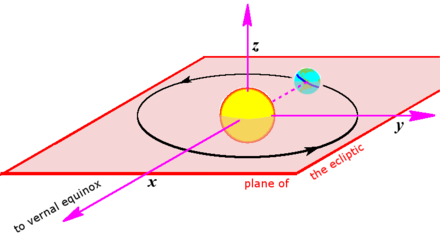
\includegraphics[width=0.8\textwidth]{heliocentric_ecliptic.png}
\caption{The Heliocentric Ecliptic Frame, courtesy of \href{https://en.wikipedia.org/wiki/Ecliptic_coordinate_system}{Wikipedia}\\
The Barycentric Ecliptic Frame is analogous, but the origin is the solar system barycenter rather than the Sun.}
\end{center}
\end{figure}

The module \tty{ra\_dec.py} handles conversions between RA/Dec and the direction $\uvec$ in the barycentric mean ecliptic (BME) frame.
The two workhorse functions are named \tty{radedc2dir} and \tty{dir2radec}.
The hard work in getting all of this to work comes in understanding the ideas of the coordinate systems and developing tests.
Once you know what everything means and how to test that the implementation is right, it amounts to just a few lines of code.
The \tty{astropy SkyCoordinate} class is aware of both the ICRF and the BME frames.
In order to transform between the two coordinate frames, we need only instantiate a \tty{SkyCoordinate} of the required type, 
and ask \tty{astropy} to transform it for us.
It's so easy I will include a code snippet to give the flavor; this is from \tty{radec2dir}:
\begin{lstlisting}[style=CodeSnippet]
obs_icrs = astropy.SkyCoord(ra=ra, dec=dec, obstime=obstime, frame=ICRS)
obs_ecl = obs_icrs.transform_to(BarycentricMeanEcliptic)
u = obs_ecl.cartesian.xyz
\end{lstlisting}

How can we test that all of this is working? 
By comparing my calculations to those done by the JPL.
At first I struggled to reconcile my results.
I downloaded the computed position of Earth and Mars from JPL as well as the RA/Dec predicted by JPL for an imaginary observer at Earth geocenter.
When I compared the JPL results to my own, they did not match,
I eventually realized that the JPL calculation is accounting for light delay.
In the next section, I wil explain this calculation and demonstrate that my results are consistent with JPL.

\section{Computing a Direction $\vec{u}$ from Position $\vec{q}$ and Velocity $\vec{v}$}
\label{section_pos_vel_to_dir}
Suppose we have computed the position $\qearth$ and $\qast$ where we believe the Earth and an asteroid are at the same time $t$.
Can we compute the direction $\uvec$ from the Earth to the asteroid by simply subtracting the poitions and normalizing them, i.e. by
$$ \uvec \stackrel{?}{=} \frac{\qast - \qearth}{\norm{\qast - \qearth}}$$
The answer is no! This fails to account for the finite speed of light.
The photons arriving at the observatory at the observation time $t_1$ were not emitted at $t_1$; they were emitted in the past, at time $t_0$.
\begin{figure}[hbt!]
\begin{center}
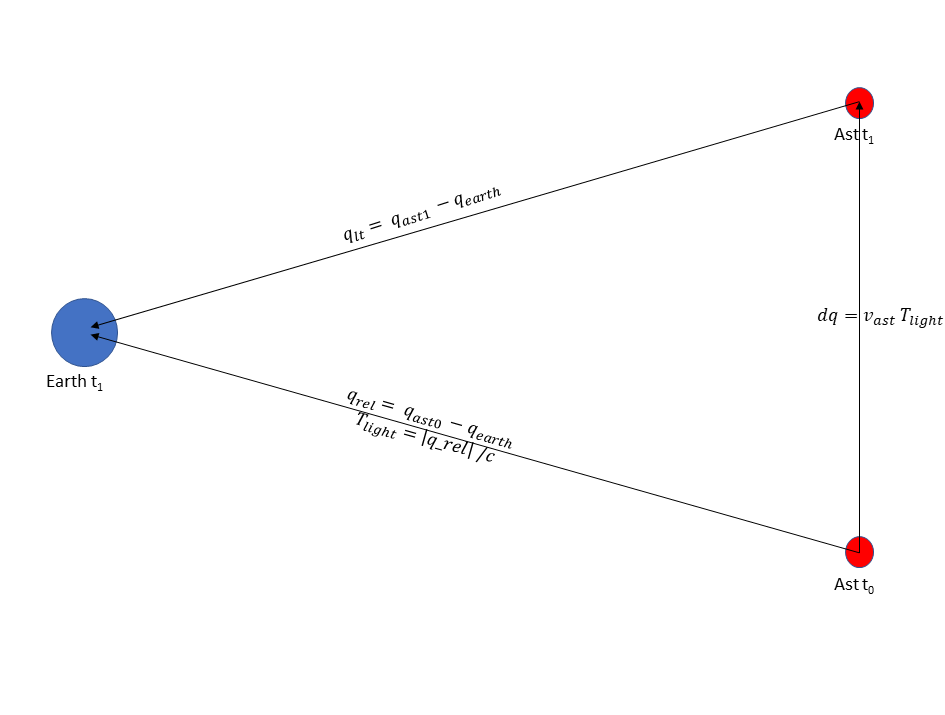
\includegraphics[width=0.8\textwidth]{light_time.png}
\caption{Computing the Apparent Direction from Earth to an Asteroid, Accounting for the Speed of Light}
\end{center}
\end{figure}
It's straightforward to calculate a correction that is accurate to first order once we draw a picture.
It requires that we know both the predicted position and the predicted velocity of the asteroid at time $t_1$.
\begin{align*}
\mathbf{q}_{\mathrm{rel}} &= \qast - \qearth \\
T_{\mathrm{light}} &= \norm{ \mathbf{q}_{\mathrm{rel}} } / c \\
\Delta \qast &= \vvec_{\mathrm{ast}} \cdot T_{\mathrm{light}} \\
\mathbf{q}_{\mathrm{lt}} &= \mathbf{q}_{\mathrm{rel}} - \Delta \qast \\
\uvec &= \mathbf{q}_{\mathrm{lt}} / \norm{\mathbf{q}_{\mathrm{lt}}}
\end{align*}
Here $c$ is the speed of light as usual.

One slightly counterintuitive fact is that we don't need to know or account for the speed of the Earth, 
or compute the relative velocity of the asteroid to the Earth. 
Why is this?
We are performing all of our calculations in the barycentric mean ecliptic frame.
This is very nearly an inertial frame of reference, so physics behaves ``nicely'' and everything works as expected.
The only small departures from this frame being inertial are due to the orbit of the solar system around the Milky Way
and the acceleration of the Milky Way in the entire universe.
If we used a different reference frame, e.g. the heliocentric frame, we would make errors due to the acceleration of this frame 
unless we accounted for them, which would be equivalent to the calculations shown here.
In the BME frame, we have determined the positions of both the Earth and the asteroid at the instant $t_1$ at which 
photons landed on the detector of the observatory.
To calculate the direction from which these photons arrived in the BME frame, we need only know where the asteroid was at the moment
$t_0$ when photons emitted from it would have arrived at $t_1$.
This calculation of an astrometric direction is implemented in the function \tty{astrometric\_dir}, also in \tty{ra\_dec.py}.
It takes as inputs \tty{q\_body}, \tty{v\_body} and \tty{q\_obs}, and returns the astrometric direction $\uvec$
from the observer to the body accounting for light time.

It's worth pointing out here that a more fully correct description would be given by solving
$$ \norm{\qearth(t_1) - \qast(t_0)} = c \cdot (t_1 - t_0) $$
This is the approach taken by the astronomy library \tty{SkyField}, which solves this equation iteratively.
Each iterative step matches the first order solution shown above.
For the purpose of this problem, the light time between an asteroid and the Earth will typically be on the order of 20 minutes or so.
(The speed of light in AU / minutes is 0.120, so 20 minutes of light travel covers 2.4 AU).
This is short enough time interval that approximating the motion of the asteroid as linear is highly accurate.

We can also use this approach to approach to make a back of the envelope estimate of the errors we might make if 
we disregarded the light time adjustment
Suppose an asteroid has $a=3$, so by Kepler's thrid law this body would have an orbital period of $3^{3/2} \approx 5.2$ years.
At a time when this asteroid is 3.0 AU from Earth, the light time would be 25 minutes, which workds out to 2.20E-4 of its orbital period.
Converting this into degrees is a multiplication by 360, and into arc seconds a further multiplication by 3600.
I estimate that ignoring light time could lead in this case to errors on the order of 285 arc seconds 
if the asteroid were moving perpendicular to its displacement to Earth.
While that's close enough to aim an amateur's optical telescope, it's a catastrophic error here.

There is one more correction we need to account for: the position of the observatory on the surface of the Earth, or ``topos''.
Our integration of the solar system gives us $\qearth$, the position of the Earth's center of mass in the BME as a function of time.
But our observatory of course sits on the surface of the earth, not at the center.
It would be too hot in the center, plus you couldn't see anything from there.
Fortunately this is another well studied problem that is handled well by mature software libraries.
I spent a lot of time trying to get a solution working based on the implementation in \tty{astropy},  but I simply could not get it to work.
Eventually I gave up and decided to use \tty{SkyField} instead.
The function \tty{calc\_topos} in \tty{ra\_dec.py} computes the topos adjustment at a named observatory site as of a vector of times.
Currently the only observatory site required is Palomar mountain in California.
The topos correction is a pair of corrections $\Delta \qvec_{\mathrm{topos}}$ and $\Delta \vvec_{\mathrm{topos}}$ such that
$$\qobs = \qearth + \Delta \qvec_{\mathrm{topos}}$$
The spline is generated with the following code snippet (slightly edited for brevity)
\begin{lstlisting}[style=CodeSnippet]
obsgeoloc = SkyField.EarthLocation.of_site(site_name))
longitude, latitude, height = obsgeoloc.geodetic
topos = SkyField.Topos(latitude=latitude, longitude=longitude, elevatiom=elevation)
dq_topos = topos.at(obstime_sf).ecliptic_position().au.T * au
\end{lstlisting}

The function \tty{qv2dir} combines the capabilities of \tty{astrometric\_dir} and \tty{calc\_topos}.
It takes as inputs \tty{q\_body}, \tty{v\_body}, \tty{q\_earth}, \tty{obstime\_mjd} and \tty{site\_name}.
It returns the astrometric direction from an observer at the named site on earth, 
to a body with the victor position and velocity vectors aligned with the observation times.

The functions described above are based on \tty{numpy} arrays and run normally on the CPU.
I also created a custom Keras Layer in TensorFlow that performs these calculations called \tty{AsteroidDirection}.
At initialization, an \tty{AsteroidLayer} requires an array \tty{ts} of MJDs, the row lengths for each observation in the batch, and the site name.
The main \tty{call} method of this layer accepts seven inputs: the orbital elements including the epoch, namely
$(a, e, i, \Omega, \omega, f, t_0)$.
It returns the predicted astrometric direction $\uvec$ from the named observatory to an asteroid with these orbital elements.
This is the core layer that is used to predict directions to candidate orbital elements during the asteroid search.

We are now ready to review the demonstration that my calculations are consistent with JPL and SkyField.
You can follow this demonstration interactively in the Jupyter notebook 
\tty{03\_RA\_DEC.ipynb} in the \tty{jupyter} directory of the project repository.
I downloaded from Horizons a data set with with the positions and velocities of Earth and Mars.
These sets contained 29,317 rows spanning a 10 year period from 2010-01-01 to 2020-01-01 sampled at 3 hour intervals.
I also downloaded from Horizons what they refer to as ``observer'' calculations including a RA/Dec.
I specified an observer location at Palomar Mountain, which is a preset observatory in Horizons.
The SkyField calculations use a slick end to end capability to predict where an observer would see an object.
It uses a downloaded JPL ephemeris file, but is otherwise a self contained calculation that is independent from both JPL and my calculations.

I compared my calculations to two sources: JPL and SkyField, as well as comparing SkyField to JPL.
The angular distance between two directions on the unit circle can be calculated with a simple formula that I will review later.  
For very small distances, the angular difference in radians is equal to the Cartesian difference between the two direction
vectors $\uvec_1$ and $\uvec_2$ on the unit sphere in $\R^3$.

Here is a table summarizing the mean difference between Horizons, SkyField and my calculations:
\begin{table}
\begin{centering}
\begin{tabular}{|c | c|}
\hline
Sources & Difference \\
\hline
SKY vs. JPL & 1.598 \\
MSE vs. JPL & 1.604 \\
MSE vs. SKY & 0.027 \\
\hline
\end{tabular}
\caption{Mean differences between JPL, SkyField, and my calculations (MSE) in Arc Seconds\\
My results are essentially identical to SkyField.  Both SkyField and I disagree with JPL by 1.6 arc seconds.}
\end{centering}
\end{table}
My results are substantially identical to SkyField, to the miniscule tolerance of 0.027 arc seconds.
Both SkyField and I differ a tiny bit from JPL, to the tune of 1.6 arc seconds.

I did some further tests, this time comparing my predicted directions from Earth to the first 16 asteroids 
with the results of applying my \tty{radec2dir} function to the RA/Dec quoted by JPL,
with the directions I predicted using the integrated orbits.  In pseudocode, the test looks like this:
\begin{align*}
\uvec_{\mathrm{JPL}} &= \tty{radec2dir(RA\_JPL, DEC\_JPL)} \\
\uvec_{\mathrm{MSE}} &= \tty{qv2dir(q\_ast\_MSE, v\_ast\_MSE, q\_earth\_MSE, 'palomar')}
\end{align*}
This test is exercising both the integration and the angle conversion.
On 10 years of daily data for 16 asteroids, the root mean squared error is \textbf{\emph{0.873 arc seconds.}}

\section{Predicting the Apparent Magnitude of an Asteoid}
\label{section_mag}
\todo{FILL THIS IN}

\section{Conclusion}
\label{section_conclusion}
I have presented in this chapter the calculations required to determine the astromentric direction 
of an asteroid observed from earth given its orbital elements.
This calculation takes into account the time for light to travel from the asteroid to the Earth
and the position of the observatory on the Earth's surface.
I have tested these calculations against two independent sources, NASA Horizons and the SkyField astronomy library.
I have demonstrated that my results are within 1.0 arc second of NASA and substantially identical to SkyField to within 0.01 arc seconds.
Finally, I have demonstrated a high speed TensorFlow implementation of these calculations in the \tty{AsteroidDirection} layer.
The TensorFlow model can predict astrometric directions of a set of candidate orbital elements 
along with the derivatives of these predicted directions with respect to the six orbital elements.
